\documentclass[12pt]{article}
\usepackage[margin=1in]{geometry} 
\usepackage{amsmath,amsthm,amssymb,amsfonts}
\usepackage{tikz}
 
\newcommand{\N}{\mathbb{N}}
\newcommand{\Z}{\mathbb{Z}}
 
\newenvironment{problem}[2][Problem]{\begin{trivlist}
\item[\hskip \labelsep {\bfseries #1}\hskip \labelsep {\bfseries #2.}]}{\end{trivlist}}
%If you want to title your bold things something different just make another thing exactly like this but replace "problem" with the name of the thing you want, like theorem or lemma or whatever
 
\begin{document}
 
%\renewcommand{\qedsymbol}{\filledbox}
%Good resources for looking up how to do stuff:
%Binary operators: http://www.access2science.com/latex/Binary.html
%General help: http://en.wikibooks.org/wiki/LaTeX/Mathematics
%Or just google stuff
 
\title{Discrete Math 2 HW 1}
\author{Ben Awad}
\maketitle
 
\begin{problem}{9.1.6}
\end{problem}
c. 

Reflexive proof:

1. $x - x = 0$ where x is a real number (algebra)

2. 0 can be represented as $\frac{0}{1}$ and is therefore a rational number (defintion of rational)

3. Therefore for all real x, (x, x) is in the relation

Symmetric proof:

1. Assume $x - y = \frac{a}{b}$ where x, y are real numbers and a, b are integers (definition of rational)

2. $-\frac{a}{b} = y - x$ (algebra)

3. $-\frac{a}{b} = 0 - \frac{a}{b} = \frac{0}{b} - \frac{a}{b} = \frac{0-a}{b}$ (algebra)

4. $k = 0-a$ where k is some integer (closure) 

5. $\frac{k}{b} = y - x$ (algebra)

6. Therefore, if (x, y) is in the relation, (y, x) must also be in the relation

Not anti-symmetric because (10, 5) and (5, 10) are in the set and $10 \neq 5$

Transitive proof:

1. Let $x - y = \frac{a}{b}$ where x, y are real numbers and a, b are integers (definition of rational)

2. Let $y - z = \frac{c}{d}$ where y, z are real numbers and c, d are integers (definition of rational)

3. $x = \frac{a}{b} + y$ (algebra)

4. $-z = \frac{c}{d} - y$ (algebra)

5. $(\frac{a}{b} + y) + (\frac{c}{d} - y) = x - z$ (algebra)

6. $\frac{a}{b} + \frac{c}{d} = x - z$ (algebra)

7. $x - z = \frac{a}{b} + \frac{c}{d} = \frac{a*d}{b*d} + \frac{c*b}{b*d} = \frac{a*d+c*b}{b*d} = \frac{k}{h}$ for some integer k, h (algebra, closure)

8. Since k, h are integers $\frac{k}{h}$ is rational (definition of rational)

8. Therefore for (x, z) are in the relation and the relation is transitive
\newline
d.

Not reflexive because (5, 5) is not in the set because $5 \neq 2*(5)$

Not symmetric because (10, 5) is in the set $10 = 2*(5)$, but (5, 10) is not in the set $5 \neq 2*(10)$

Anti-symmetric proof:

1. $x = 2y$ (definition (x, y))

2. $y = 2x$ (definition (y, x))

3. $y \neq 4y$ (algebra)

4. The first part of the implication is always false therefore the whole thing is always true

Not transitive because (4, 2) is in the set $4 = 2*(2)$ and (2, 1) is in the set $2 = 2*(1)$, but (4, 1) is not in the set $4 \neq 2*(1)$

\begin{problem}{9.1.32}
\end{problem}

$R \circ S$: \{(3, 2), (3, 3), (4, 4), (2, 3), (4, 3), (2, 2), (3, 4)\}

$S \circ R$: \{(1, 2), (1, 1), (2, 1), (2, 2)\}

\begin{problem}{9.1.36}
\end{problem}
c. $\{ (a, b) \in R^2\}$
\newline
e. $\{ (a, b) \in R^2 | a > b\}$

\begin{problem}{9.6.10}
\end{problem}

Not partial order because it is not transitive. c $\rightarrow$ d, d $\rightarrow$ b, but c does not go to b

\begin{problem}{9.6.22}
\end{problem}

c.

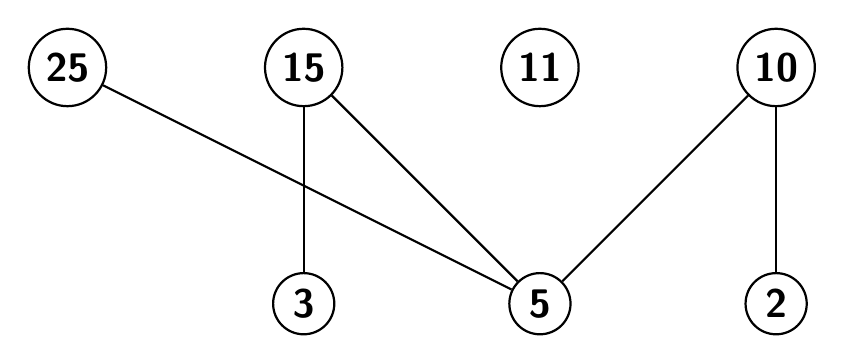
\begin{tikzpicture}[auto, node distance=3cm, every loop/.style={},
                    thick,main node/.style={circle,draw,font=\sffamily\Large\bfseries}]

  \node[main node] (25) {25};
  \node[main node] (15) [right of=25] {15};
  \node[main node] (11) [right of=15] {11};
  \node[main node] (10) [right of=11] {10};
  \node[main node] (3) [below of=15] {3};
  \node[main node] (5) [right of=3] {5};
  \node[main node] (2) [right of=5] {2};

  \path[every node/.style={font=\sffamily\small}]
  (25) edge node [right] {} (5)
  (15) edge node [right] {} (5)
  (10) edge node [left] {} (5)
  (2) edge node {} (10)
  (3) edge node {} (15)
  ;
\end{tikzpicture}

\begin{problem}{9.6.26}
\end{problem}

\end{document}
